\chapter{PILCO-style offline PI tuning and expected fuel reversal}
\label{ch:policy}
This chapter studies a restricted adaptation of probabilistic policy evaluation, not a new PILCO algorithm. A frozen quadratic supplies feedforward, an offline GP predicts dynamics, and two PI gains are optimized numerically. The first experiment and the later ringing penalty are retained together so that the repair of an aggressive policy is not mistaken for a demonstrated advantage over conventional PI. The relationship to original PILCO and CAPS is evaluated in Chapter~\ref{ch:literature}.

\section{PILCO-style policy learning: full derivation and first results}
\textit{Archived October study. All simulations, searches, and checks described below predate this report.}\par

\subsection*{Chapter overview}
A Gaussian-process (GP) transition model and analytic Gaussian moment propagation are used to optimize a proportional-integral controller around an existing quadratic feedforward map. The benchmark is the previous 9250 rpm, sea-level, ISA-zero test with shaft-load pulses. Three historical controllers and the initial PI policy provide comparators. The selected gains are frozen before new nonlinear T-MATS simulations at 10\% and 5\% load amplitudes. This implementation is a PILCO-style, offline, single-model policy-improvement experiment: it uses numerical policy gradients, a fitted linear mean, a shared-kernel GP subset, and an expected quadratic cost. It is not an exact reproduction of the original PILCO training loop. All reported plant metrics come from saved nonlinear simulation traces, not GP rollout predictions.

\subsection{Experiment, provenance, and main result}
The chosen test is the most recent fixed-operating-point study in this workspace. The reference is 9250 rpm, altitude is 0 m, ISA deviation is 0 K, and Mach number is zero. Each simulation includes 60 s preparation and 90 s evaluation. The sample period is $h=0.015$ s. Turbine trim power is 15376.79195 hp; the 10\% disturbance is 1537.67919 hp. Relative to the evaluation start, load pulses occupy $[10.005,15)$, $[30,40.005)$, and $[60,75)$ s. Five-percent validation halves only the pulse magnitude.

The existing base PI, original Poly2, and retuned Poly2 traces are read from the previous study without alteration. The latter two include acceleration feedback (PID-like), so they are explicitly labelled as such. The new policy uses ordinary sensed-speed error and no derivative feedback.

The new nonlinear simulation has speed RMSE 1.1973 rpm, peak error 14.389 rpm, and fuel ringing 14.8252 lbm/s. Compared with retuned Poly2, tracking RMSE falls by 22.6\%, but ringing grows to 11.4 times its previous value. This is a tracking--actuation tradeoff, not an overall improvement.

\paragraph{Scope of the feedforward claim.} The quadratic coefficients are frozen from the prior inverse fit. PILCO learns the two PI gains, not the fifteen polynomial coefficients. At one fixed speed and ambient condition, feedforward is a constant and its offset is absorbed by bumpless integral initialization. Consequently this benchmark cannot identify a quadratic-map advantage over other constant feedforward values. The static map also slightly extrapolates: 9250 rpm is below its previous training-speed minimum of approximately 9264.23 rpm.

\subsection{Step 1: write the deployed control law}
Let $N_s$ denote sensed shaft speed, $r$ the governed reference, $T$ inlet temperature in kelvin, and $P$ inlet pressure in kPa. The old inverse model uses inputs $v=[N,\dot N,T,P]^\top$, standardized as $z_j=(v_j-\bar v_j)/s_j$. Its full quadratic is
\begin{equation}
 p_2(v)=c_0+\sum_{j=1}^4c_jz_j+\sum_{j=1}^4c_{jj}z_j^2+\sum_{i<j}c_{ij}z_iz_j.
\end{equation}
There are $1+4+4+6=15$ coefficients. Setting desired acceleration to zero defines static feedforward. The actual controller is
\begin{align}
 u_{\rm ff,k}&=p_2(r_k,0,T_k,P_k), &e_k&=r_k-N_{s,k},\\
 u_k^*&=u_{\rm ff,k}+K_pe_k+I_k, &u_k&=\operatorname{clip}(u_k^*,0.2,4),\\
 I_{k+1}&=I_k+hK_ie_k &&\text{when integration is permitted.}
\end{align}
Fuel is measured in lbm/s, $K_p$ in (lbm/s)/rpm and $K_i$ in (lbm/s)/(rpm s). Conditional integration permits an update if $(u^*<4\text{ or }e<0)$ and $(u^*>0.2\text{ or }e>0)$. Before 45 s the old controller supplies the command and the new integral tracks $I=u_{\rm old}-u_{\rm ff}-K_pe$. This gives a bumpless handover. Existing plant, sensor, request governor, load profile, solver and fuel limits are inherited by the new model copy.

\subsection{Step 2: construct the dynamics-learning state}
Use a dimensionless augmented state and a normalized load:
\begin{equation}
 x=\begin{bmatrix}(N-9250)/20\\(N-N_s)/5\\(I-I_0)/0.3\end{bmatrix},\quad
 d=\frac{P_{\rm load}}{1537.6791946},\quad I_0=u_0-u_{\rm ff}.
\end{equation}
The trim fuel $u_0=1.39529998$ lbm/s. The second state represents sensor lag; discarding it would make fast feedback dynamics less nearly Markov. At fixed reference,
\begin{equation}
 \tilde u=(u-u_0)/0.3=b^\top x,\qquad
 b^\top=\left[-\frac{20K_p}{0.3},\frac{5K_p}{0.3},1\right].
\end{equation}
The GP input is $z=[x_1,x_2,\tilde u,d]^\top=B x+a(d)$ and its output is the two physical-state increments $y=[\Delta x_1,\Delta x_2]^\top$. The integrator transition is known exactly, so learning it would waste data. With
\begin{equation}
 D=\begin{bmatrix}1&0&0\\0&1&0\\-20hK_i/0.3&5hK_i/0.3&1\end{bmatrix},\quad
 E=\begin{bmatrix}1&0\\0&1\\0&0\end{bmatrix},\qquad x^+=Dx+Ey,
\end{equation}
the feedback integral remains correlated with the turbine state during planning.

\subsection{Step 3: fit the probabilistic transition model}
Training uses transitions from the first two pulses of each historical controller: absolute windows $[69.9,78]$ and $[89.9,103]$ s. There are 4242 transitions. The third-pulse window $[119.9,138]$ s is held out for one-step dynamics checks. These trajectories share a deterministic plant and operating point; this is a temporal split, not independent hardware validation.

Fit a linear mean by least squares on training data only, $m(z)=a+Az$, and standardize each residual output with scale $s_j$. A deterministic farthest-point selection retains 40 representative GP inputs. For both standardized residual outputs, use the shared squared-exponential kernel
\begin{equation}
 k(z,z')=\sigma_f^2\exp\left[-\tfrac12(z-z')^\top\Lambda^{-1}(z-z')\right],\qquad
 \Lambda=\operatorname{diag}(\ell_1^2,\ldots,\ell_4^2).
\end{equation}
Let $K_n=K+\sigma_n^2\mathcal I+10^{-9}\mathcal I$ and let $R$ contain standardized residuals. Cholesky solves minimize the summed negative log marginal likelihood, up to constants:
\begin{equation}
 \mathcal L=\tfrac12\operatorname{tr}(R^\top K_n^{-1}R)+\frac{2}{2}\log|K_n|,\qquad \beta=K_n^{-1}R.
\end{equation}
The hyperparameter bounds in log units are $[-1,4]$ for length scales, $[-3,3]$ for signal standard deviation and $[-7,0]$ for noise standard deviation. Conditional on a deterministic input, residual outputs are independent and share covariance hyperparameters. Uncertain inputs induce output cross-covariance. The linear mean is treated as fixed: uncertainty in its estimated coefficients is not integrated out.

\subsection{Step 4: propagate a Gaussian through the policy}
Suppose $x\sim\mathcal N(\mu,\Sigma)$. For the unsaturated policy, the input moments are exact:
\begin{equation}
 m_z=B\mu+a(d),\qquad S_z=B\Sigma B^\top,\qquad C_{xz}=\Sigma B^\top.
\end{equation}
The load is a known deterministic scenario input during planning, not a measured feedforward input to the deployed policy. A full Gaussian may mathematically cross the fuel limits. Planning here uses the unsaturated affine policy; the nonlinear plant evaluation applies clipping and anti-windup. This is a local approximation, justified only to the extent that the evaluated commands remain inside the limits.

\subsection{Step 5: derive exact uncertain-input GP moments}
Write $m=m_z$, $S=S_z$, and let $z_i$ denote training inputs. Completing the square in the Gaussian integral of one kernel gives
\begin{align}
 q_i&=\int k(z,z_i)\mathcal N(z\mid m,S)\,dz\\
 &=\sigma_f^2\frac{|\Lambda|^{1/2}}{|S+\Lambda|^{1/2}}
 \exp\left[-\tfrac12(z_i-m)^\top(S+\Lambda)^{-1}(z_i-m)\right].
\end{align}
For two kernels, define $c_{ij}=(z_i+z_j)/2$ and $\delta_{ij}=z_i-z_j$. Their product separates into a distance factor and a Gaussian centered at $c_{ij}$. Therefore
\begin{align}
 Q_{ij}&=\E[k(z,z_i)k(z,z_j)]\\
 &=\sigma_f^4\exp[-\tfrac14\delta_{ij}^\top\Lambda^{-1}\delta_{ij}]
 \frac{|\Lambda/2|^{1/2}}{|S+\Lambda/2|^{1/2}}\nonumber\\
 &\hspace{7mm}\cdot\exp[-\tfrac12(c_{ij}-m)^\top(S+\Lambda/2)^{-1}(c_{ij}-m)].
\end{align}
Let $g$ be the standardized residual GP output. The law of total expectation and total covariance now give
\begin{align}
 \bar g&=\beta^\top q,\\
 V_g&=\beta^\top Q\beta-\bar g\bar g^\top+
 \mathcal I\left[\sigma_f^2-\operatorname{tr}(K_n^{-1}Q)+\sigma_n^2\right].
\end{align}
The last term includes observation/model-residual noise in each predicted transition. Propagating this as temporally independent noise does not represent a single fixed GP function sample across the entire horizon. This standard moment-propagation approximation can accumulate model uncertainty differently from trajectory sampling.

The Gaussian kernel identity also yields
\begin{equation}
 G=(S+\Lambda)^{-1}\sum_i(z_i-m)q_i\beta_i^\top H,
 \qquad H=\operatorname{diag}(s_1,s_2).
\end{equation}
Then $\Cov(z,Hg)=SG$. Restoring the linear mean and residual scales,
\begin{align}
 \bar y&=a+Am+H\bar g,\\
 V_y&=ASA^\top+HV_gH+ASG+G^\top SA^\top,\\
 C_{xy}&=C_{xz}(A^\top+G).
\end{align}
The cross terms matter: dropping $C_{xy}$ loses the dependence between current state and predicted state increment. All inverses above involve a positive-definite kernel length-scale matrix added to $S$, so a singular $S$ from deterministic scenario inputs is allowed.

\subsection{Step 6: close the moment recursion}
Substitution into $x^+=Dx+Ey$ gives
\begin{align}
 \mu^+&=D\mu+E\bar y,\\
 \Sigma^+&=D\Sigma D^\top+EV_yE^\top+DC_{xy}E^\top+EC_{xy}^\top D^\top.
\end{align}
Each transition is then approximated by a Gaussian with these moments. This preserves first and second moments of the one-step mapping under the Gaussian input assumption; it does not preserve multimodality of the true multistep distribution. Initial planning moments are $\mu_0=0$ and $\Sigma_0=\operatorname{diag}(10^{-6},10^{-6},10^{-8})$.

\subsection{Step 7: derive and optimize the expected cost}
For a 5 s planning horizon at the same 15 ms sample period, a unit load pulse is applied for $1\le t<2.5$ s. The objective is
\begin{align}
 J(\theta)&=h\sum_k\E[x_{1,k}^2+0.01\tilde u_k^2]\\
 &=h\sum_k\left[\mu_{1,k}^2+\Sigma_{11,k}+0.01\{(b^\top\mu_k)^2+b^\top\Sigma_kb\}\right].
\end{align}
Use $\theta=[\log K_p,\log K_i]^\top$, so gains remain positive. Bounds are $0.005\le K_p\le0.07$ and $0.01\le K_i\le0.25$. The initial policy is $(0.025,0.05)$. L-BFGS-B repeatedly evaluates the complete Gaussian rollout and estimates parameter gradients numerically. The conceptual chain rule is
\begin{equation}
 \frac{dJ}{d\theta}=\sum_k\left(\frac{\partial J}{\partial\mu_k}\frac{d\mu_k}{d\theta}+\frac{\partial J}{\partial\Sigma_k}:\frac{d\Sigma_k}{d\theta}+\frac{\partial J}{\partial\theta}\right).
\end{equation}
For implementation, this derivative is approximated by finite differences of the full objective rather than hand-coded analytic sensitivities. The learned result is
\begin{equation}
 \boxed{K_p=0.06460568,\qquad K_i=0.17102610,\qquad K_d=0.}
\end{equation}
Expected cost changes from 0.464463 to 0.141314. This cost is dimensionless and is not the reported full-test speed RMSE or fuel-ringing metric. Gains are frozen immediately after optimization; no 5\% validation result is used in selection.
\begin{figure}[H]\centering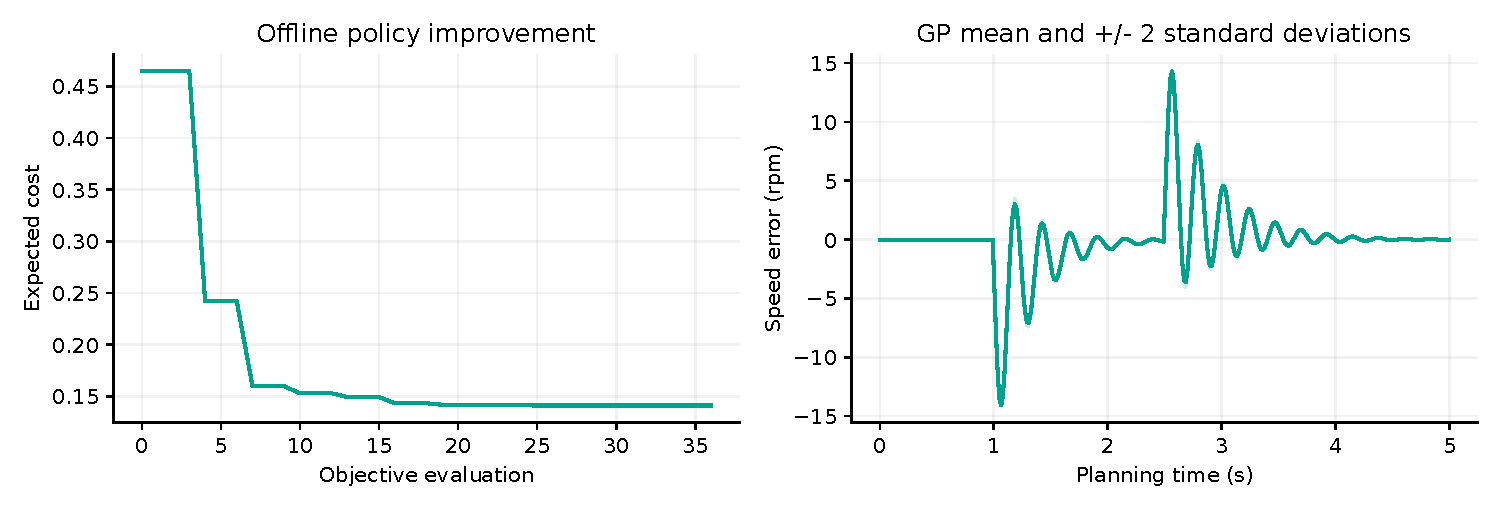
\includegraphics[width=\linewidth,height=.68\textheight,keepaspectratio]{late0_learning.pdf}\caption{Policy-search objective and GP planning response. The shaded interval is model uncertainty, not a certified plant confidence band.}\end{figure}

\subsection{Step 8: nonlinear plant comparison and independent checks}
All three new simulations use the copied T-MATS plant: selected policy at 10\%, selected policy at 5\%, and initial quadratic-feedforward PI at 10\%. Historical traces supply the three earlier comparators. The initial-policy ablation helps distinguish gain learning from merely adding a constant feedforward value. File hashes and replay checks are saved with the study.

\begin{table}[H]\centering\small\begin{tabular}{lrrrr}\toprule Controller & RMSE & Peak & Ringing & Settling\\ & rpm & rpm & lbm/s & s\\\midrule
Base PI & 2.4209 & 21.406 & 2.0702 & 2.475 \\
Original Poly2 + PID & 1.6658 & 14.113 & 1.6968 & 1.365 \\
Retuned Poly2 + PID & 1.5461 & 15.825 & 1.2990 & 0.930 \\
PILCO FF+PI & 1.1973 & 14.389 & 14.8252 & 1.920 \\\bottomrule\end{tabular}\caption{10\% load-amplitude comparison.}\end{table}
\begin{table}[H]\centering\small\begin{tabular}{lrrrr}\toprule Controller & RMSE & Peak & Ringing & Settling\\ & rpm & rpm & lbm/s & s\\\midrule
Base PI & 1.1692 & 10.392 & 1.0583 & 2.115 \\
Original Poly2 + PID & 0.8018 & 6.969 & 0.9005 & 1.260 \\
Retuned Poly2 + PID & 0.7439 & 7.806 & 0.6544 & 0.870 \\
PILCO FF+PI & 0.5930 & 7.008 & 7.9471 & 1.695 \\\bottomrule\end{tabular}\caption{5\% load-amplitude comparison.}\end{table}

RMSE uses every sample in $[60,150]$ s. Peak error is maximum absolute speed error in that interval. IAE uses the same rectangular sample sum as the prior report. Fuel ringing sums, over six two-second event windows, total variation minus absolute net fuel change:
\begin{equation}
 R=\sum_{j=1}^{6}\left[\sum_{k\in W_j}|u_{k+1}-u_k|-|u_{\mathrm{last}(j)}-u_{\mathrm{first}(j)}|\right].
\end{equation}
This is a reversal metric in lbm/s, not fuel consumed. Settling requires persistent entry into $\pm0.1$ rpm until the next event. Numerical acceptance checks full duration, finite signals, positive fuel, positive surge margin, flow residual at most $10^{-9}$, fewer than 200 solver iterations, and pre-test speed within 0.1 rpm.

The analytic GP covariance agrees with a 50,000-input Monte Carlo integration to 0.31\% relative Frobenius error; input/output cross-covariance error is 1.57\%. Held-out one-step speed-increment RMSE ranges from 0.000432 to 0.000709 rpm. Independent command and integral replay errors are below $10^{-8}$. All evaluated new traces pass the existing numerical acceptance checks. The selected 10\% run has minimum surge margin 14.800\% and fuel saturation fraction 0.000\%.
\begin{figure}[H]\centering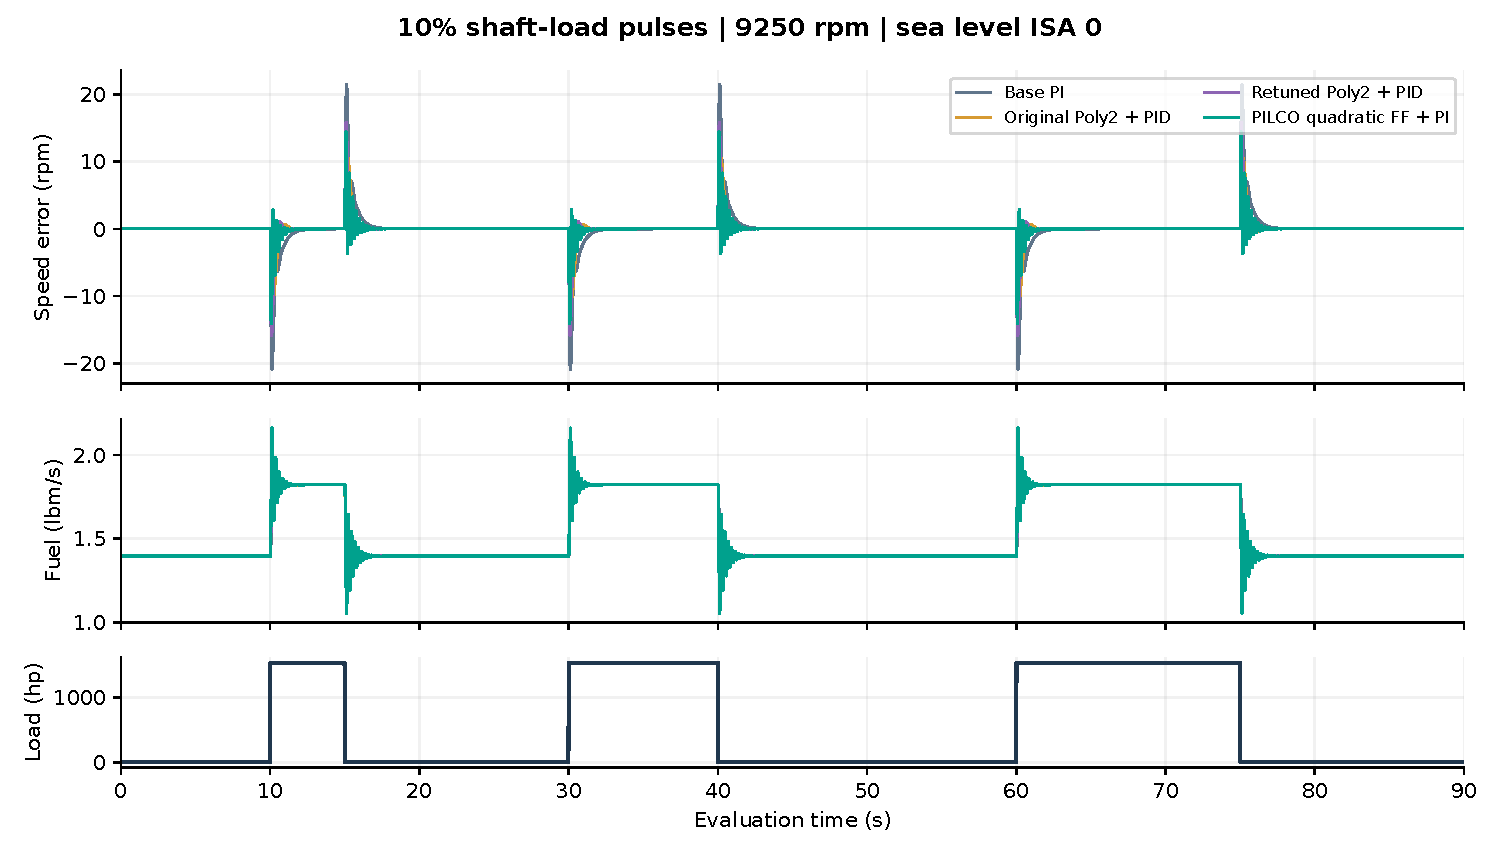
\includegraphics[width=\linewidth,height=.68\textheight,keepaspectratio]{late0_comparison_10pct.pdf}\caption{Full nonlinear 10\% benchmark. Historical methods and new controller use matching time, request and disturbance profiles.}\end{figure}
\begin{figure}[H]\centering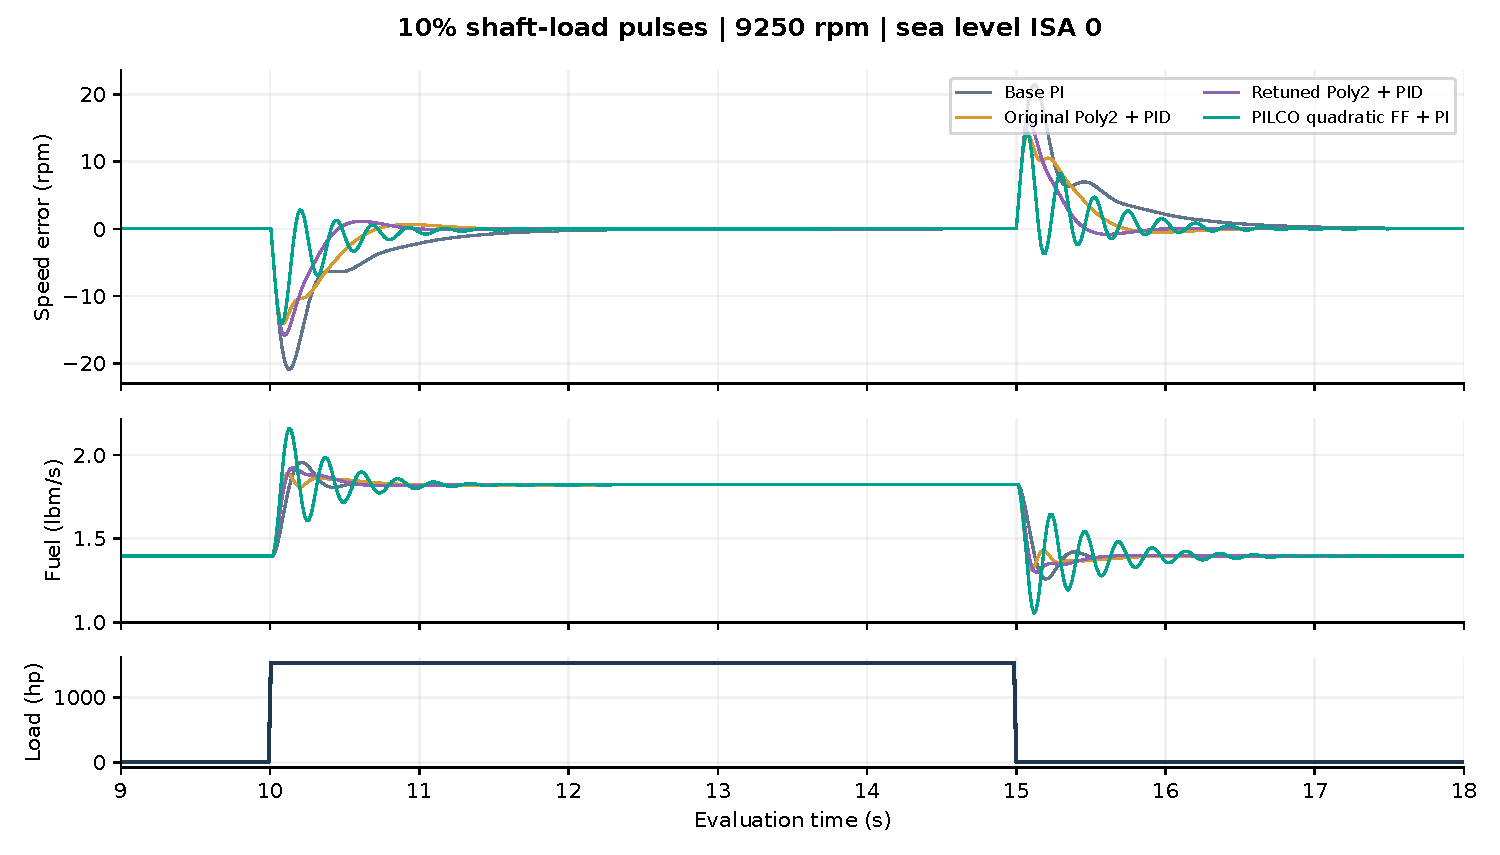
\includegraphics[width=\linewidth,height=.68\textheight,keepaspectratio]{late0_zoom_10pct.pdf}\caption{First pulse, emphasizing overshoot and command reversals. The new method is judged on these plant traces.}\end{figure}
\begin{figure}[H]\centering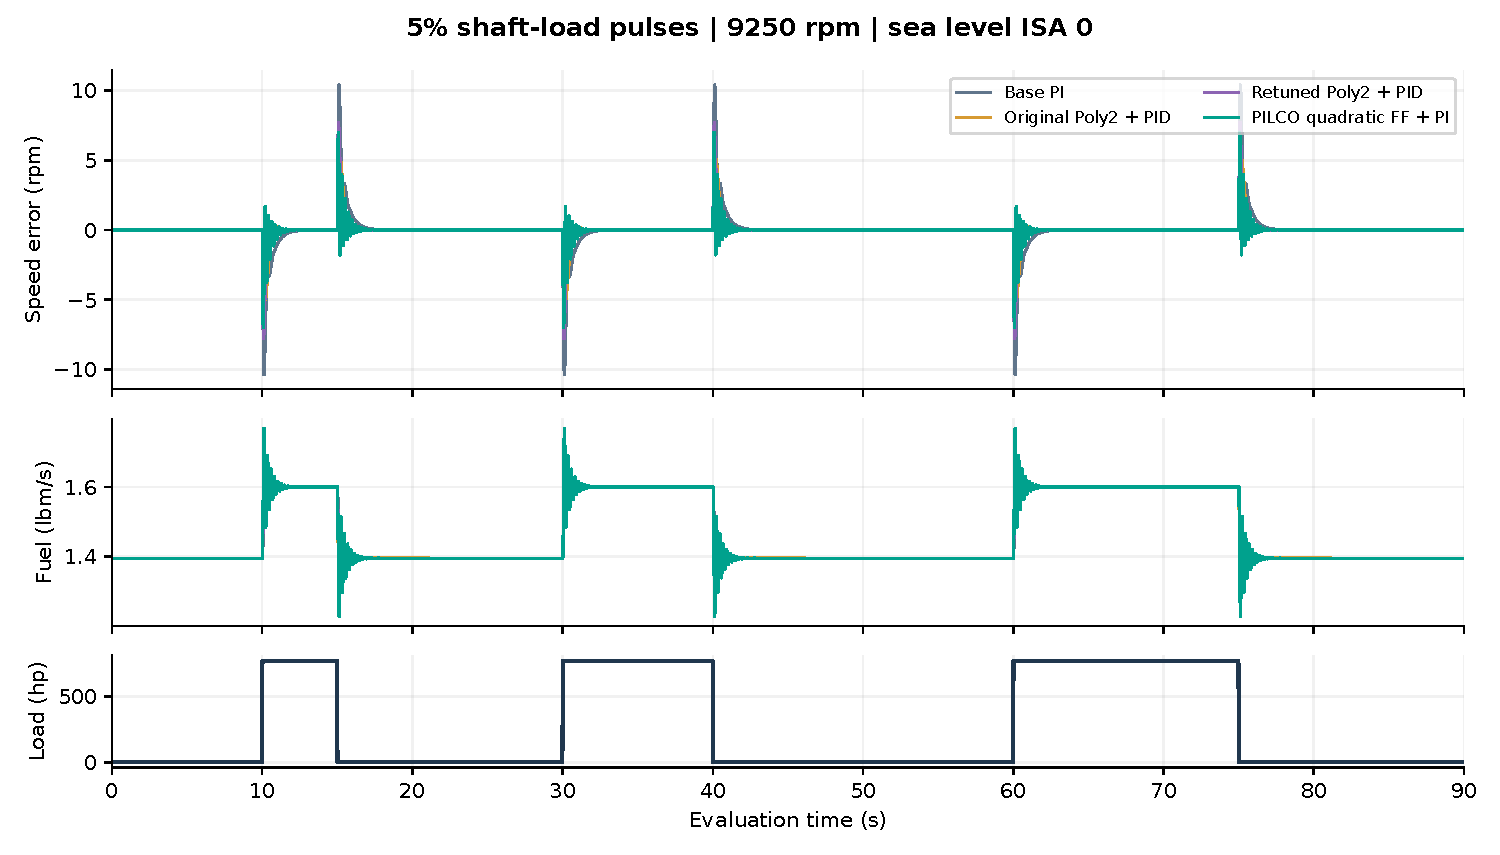
\includegraphics[width=\linewidth,height=.68\textheight,keepaspectratio]{late0_comparison_5pct.pdf}\caption{Frozen-policy 5\% amplitude validation at the same operating point.}\end{figure}

\subsection{Interpretation and limitations}
Relative to Base PI, RMSE changes by -50.5\% and ringing by +616.1\%. Relative to Retuned Poly2 + PID, RMSE changes by -22.6\% and ringing by +1041.2\%. The initial feedforward PI has RMSE 2.4406 rpm and ringing 2.0296 lbm/s. These quantities describe different tradeoffs; minimizing expected tracking cost does not directly minimize fuel reversals.

The original PILCO method uses GP dynamics, uncertainty-aware long-horizon prediction and policy search with analytic gradients~\cite{pilco}. This study retains GP moment matching but changes the policy family, cost, mean function, training source and gradient implementation. It performs one offline improvement round using existing experiments; it does not claim learning from scratch or a repeated collect--refit--improve loop. Forty representative GP points are a subset approximation, and a low held-out one-step error does not establish calibrated long-horizon uncertainty. The moment check validates the algebra against integration, not the physical accuracy of the GP.

The local state omits thermodynamic internal states; the linear mean and GP can absorb only their effects visible in the training trajectories. The deployment sensor dynamics are inherited from the plant, while learning identifies their observed effect. No guarantee of global stability, robustness at other speeds or ambient conditions, or hardware safety follows from these simulations. A multi-speed test with a frozen validation protocol would be required to assess the quadratic feedforward surface itself. The video is an animation of recorded signals; rotor speed is visually scaled and is not a blade-resolved turbine simulation.

\subsection{Reproduction and delivered files}
The source scripts are \path{pilco_tmats.py} (GP and policy learning), \path{tmats_pilco_pi_sfun.m} (deployed controller), \path{tmats_pilco_setup.m}, \path{run_tmats_pilco.m} (plant runs), and \path{build_pilco_deliverables.py} (verification, figures, paper and video). The ready-to-open model is \path{GasTurbine_PILCO_Quadratic_PI.mdl}. It requires the existing adjacent T-MATS library and the frozen fit files in this workspace.

Run Python learning first, then execute \path{run_tmats_pilco} in MATLAB R2018b or a compatible release. Finally run the artifact builder. The results directory contains policy JSON, GP parameters, search history, prediction moments, MAT/CSV plant traces, comparison metrics, replay verification and a hash manifest. The paper source and figures are included alongside the PDF. Re-running overwrites only this study's outputs; preserve them first if a second independent run is desired.



\section{Learning smoother control with an expected ringing penalty}
\textit{Archived October study. All simulations, searches, and checks described below predate this report.}\par

\subsection*{Chapter overview}
The preceding PILCO-style controller reduced speed-error RMSE but produced much larger fuel-command reversals. This study modifies policy learning to penalize expected excess total variation of fuel. A previous-command state and an event-start anchor retain the correlations needed to evaluate that penalty under Gaussian moment propagation. Seven coarse penalty weights and three intermediate refinements are optimized with the unchanged GP dynamics model and checked on the nonlinear gas-turbine plant. A declared joint tracking/ringing score selects a policy using only 10\% load tests, after which a 5\% test evaluates the frozen gains. The method remains an offline PILCO-style adaptation with numerical policy gradients and a frozen quadratic feedforward map. The report separates probabilistic predictions, plant measurements, and limitations.

\subsection{Outcome and why the objective changed}
The selected penalty is $\lambda=0.2$, with $K_p=0.02479762$ and $K_i=0.05385920$. In the nonlinear 10\% test, ringing falls by 85.9\% relative to the previous PILCO policy, from 14.8252 to 2.0838 lbm/s. Speed RMSE changes from 1.1973 to 2.3877 rpm. The smoother command therefore has a measurable tracking cost.

The previous learned gains were $K_p=0.06460568$, $K_i=0.17102610$, $K_d=0$. Their training objective rewarded small speed error and modest fuel magnitude, but neither term distinguished a smooth fuel trajectory from one repeatedly reversing around its equilibrium. A fast, aggressive PI policy could therefore score well despite oscillation. This was visible in the previous full nonlinear 10\% test: RMSE was 1.19728 rpm and ringing was 14.82523 lbm/s, compared with 1.54614 rpm and 1.29904 lbm/s for retuned Poly2 with derivative feedback.

The present change acts in \emph{policy learning}. No post-processing is applied to plant traces or video curves, and no extra low-pass filter is inserted into the fuel command. The deployed controller remains quadratic feedforward plus ordinary speed-error PI; changing its optimized gains changes the actual nonlinear plant response.

\subsection{The experiment and what is held fixed}
The reference is 9250 rpm at sea level, ISA zero and Mach zero. There are 60 s of preparation and 90 s of evaluation at $h=0.015$ s. The three 10\% shaft-load pulses occupy evaluation intervals $[10.005,15)$, $[30,40.005)$ and $[60,75)$ s. Their magnitude is 1537.67919 hp, obtained from the same 15376.79195 hp trim as the preceding studies. Validation uses 768.83960 hp with identical timing. The numerical solver, speed sensor, fuel limits, feedforward coefficients and startup procedure are unchanged.

The dynamics GP is loaded from the previous study without refitting. Its training comprises 4242 transitions from the first two pulse windows of base PI, original Poly2 and retuned Poly2. A 40-point representative subset models residuals around a fitted linear mean. The original third-pulse holdout remains outside GP fitting. However, the 10\% full-test traces now participate in penalty-weight selection; they are tuning results, not independent validation. Five-percent data are never used to choose the policy in this study.

\subsection{Step 1: the deployable controller}
For standardized inverse-model inputs $z_j=(v_j-\bar v_j)/s_j$ with $v=[N,\dot N,T,P]^\top$, retain the full quadratic
\begin{equation}
p_2(v)=c_0+\sum_{j=1}^4c_jz_j+\sum_{j=1}^4c_{jj}z_j^2+\sum_{i<j}c_{ij}z_iz_j.
\end{equation}
At each sample, the actual control law is
\begin{align}
u_{{\rm ff},k}&=p_2(r_k,0,T_k,P_k),& e_k&=r_k-N_{s,k},\\
u_k^*&=u_{{\rm ff},k}+K_pe_k+I_k,&u_k&=\operatorname{clip}(u_k^*,0.2,4),\\
I_{k+1}&=I_k+hK_ie_k&&\text{if conditional integration permits it.}
\end{align}
The integral updates if $(u^*<4\text{ or }e<0)$ and $(u^*>0.2\text{ or }e>0)$, allowing correction out of saturation. Before 45 s, the old command drives the plant and the new integral tracks $I=u_{\rm old}-u_{\rm ff}-K_pe$ for bumpless transfer. Gains have units $(\mathrm{lbm/s})/\mathrm{rpm}$ and $(\mathrm{lbm/s})/(\mathrm{rpm\,s})$.

Only $K_p$ and $K_i$ are learned. The polynomial's fifteen coefficients are fixed. At this single setpoint and ambient condition, feedforward is constant and an integral offset can compensate its value. The experiment therefore assesses PI tuning, not the benefit of the quadratic surface across speeds. The setpoint remains slightly below the old polynomial training-speed minimum of 9264.23 rpm.

\subsection{Step 2: distinguish magnitude, slew, total variation, and ringing}
Fuel magnitude describes how much fuel is commanded. Slew is the local rate $(u_k-u_{k-1})/h$. Total variation counts accumulated command motion, while excess variation removes the unavoidable net motion between endpoints:
\begin{align}
\mathrm{TV}_{a:b}(u)&=\sum_{k=a+1}^{b}|u_k-u_{k-1}|,\\
R_{a:b}(u)&=\mathrm{TV}_{a:b}(u)-|u_b-u_a|\ge0.
\end{align}
The inequality follows from the triangle inequality. For a monotone trajectory $[0,0.5,1]$, TV and net change both equal 1, so ringing is zero. For $[0,1,0,1]$, TV is 3 and net change is 1, so ringing is 2. A direct excess-TV penalty discourages reversals without penalizing a required monotone fuel transition as strongly as plain TV would.

The metric has units lbm/s because it sums changes in a fuel-flow command. It is neither integrated fuel consumption nor the integral of squared fuel slew. It is sensitive to sample rate and noise. This study keeps the sample rate fixed for every comparison. Penalizing ringing does not automatically bound peak slew: the report separately measures that quantity.

\subsection{Step 3: augment the state to preserve temporal correlation}
Use normalized physical and controller states
\begin{equation}
x=\begin{bmatrix}(N-9250)/20\\(N-N_s)/5\\(I-I_0)/0.3\end{bmatrix},\quad
I_0=u_0-u_{\rm ff},\quad\tilde u=\frac{u-u_0}{0.3}=b^\top x,
\end{equation}
where $u_0=1.39529998$ lbm/s and $b^\top=[-20K_p/0.3,\;5K_p/0.3,\;1]$ for the unsaturated fixed-reference policy. To evaluate fuel increments and endpoint changes, introduce
\begin{equation}
\xi=\begin{bmatrix}x\\p\\a\end{bmatrix},\qquad p=\tilde u_{k-1},\qquad a=\tilde u_{\rm event\ start},\qquad
\bar b=\begin{bmatrix}b\\0\\0\end{bmatrix}.
\end{equation}
The five-dimensional covariance includes the cross-covariance between current state, previous command and event-start anchor. Ignoring these correlations would generally overestimate incremental-command uncertainty. In particular,
\begin{equation}
\Var(\tilde u_k-p_k)=\Var(\tilde u_k)+\Var(p_k)-2\Cov(\tilde u_k,p_k).
\end{equation}
At the beginning of each planning event, set the anchor to the current policy output. This is a deterministic linear transformation $\xi\leftarrow T\xi$, where $T$ is identity except its fifth row is $\bar b^\top$. Thus both moments transform: $m\leftarrow Tm$ and $S\leftarrow TST^\top$. Resetting only the anchor mean would be incorrect.

\subsection{Step 4: propagate the unchanged GP and augmented moments}
The normalized GP input is
\begin{equation}
z=[x_1,x_2,\tilde u,d]^\top=B\xi+c(d),\qquad d=P_{\rm load}/1537.6791946.
\end{equation}
With $\xi\sim\mathcal N(m,S)$, its input moments and state/input cross-covariance are $m_z=Bm+c$, $S_z=BSB^\top$, and $C_{\xi z}=SB^\top$. The GP returns two increments $y=[\Delta x_1,\Delta x_2]^\top$. Integration and command memory are known transitions:
\begin{equation}
\xi^+=D\xi+Ey,\qquad
D=\begin{bmatrix}
1&0&0&0&0\\0&1&0&0&0\\-20hK_i/0.3&5hK_i/0.3&1&0&0\\
-20K_p/0.3&5K_p/0.3&1&0&0\\0&0&0&0&1
\end{bmatrix},\qquad E=\begin{bmatrix}1&0\\0&1\\0&0\\0&0\\0&0\end{bmatrix}.
\end{equation}
The fourth state becomes the current command, and the fifth retains the event anchor. The GP residual uses a shared squared-exponential kernel,
\begin{equation}
k(z,z')=\sigma_f^2\exp[-\tfrac12(z-z')^\top\Lambda^{-1}(z-z')],\qquad K_n=K+\sigma_n^2\mathcal I+10^{-9}\mathcal I.
\end{equation}
For Gaussian input, let $q_i=\E[k(z,z_i)]$, $Q_{ij}=\E[k(z,z_i)k(z,z_j)]$ and $\beta=K_n^{-1}R$, where $R$ contains standardized training residuals. Then
\begin{align}
q_i&=\sigma_f^2\frac{|\Lambda|^{1/2}}{|S_z+\Lambda|^{1/2}}
\exp[-\tfrac12(z_i-m_z)^\top(S_z+\Lambda)^{-1}(z_i-m_z)],\\
\mu_g&=\beta^\top q,\\
V_g&=\beta^\top Q\beta-\mu_g\mu_g^\top+
\mathcal I[\sigma_f^2-\operatorname{tr}(K_n^{-1}Q)+\sigma_n^2].
\end{align}
The two-kernel integral $Q$ uses the midpoint $(z_i+z_j)/2$ and covariance $\Lambda/2$; the full expression and previous validation are available in the preceding policy-learning chapter. Restoring residual output scales and the fitted linear mean yields $\mu_y,V_y,C_{\xi y}$. The recursion is
\begin{align}
m^+&=Dm+E\mu_y,\\
S^+&=DSD^\top+EV_yE^\top+DC_{\xi y}E^\top+EC_{\xi y}^\top D^\top.
\end{align}
Each propagated state is approximated as Gaussian. GP noise is treated as independent at successive transitions. This is uncertainty propagation under a model approximation, not a probabilistic safety guarantee or a temporally coherent GP function draw.

\subsection{Step 5: derive expected absolute command motion}
For a scalar Gaussian $Z\sim\mathcal N(\mu,v)$, split the integral at zero:
\begin{align}
\E|Z|&=\int_{-\infty}^0(-z)\mathcal N(z\mid\mu,v)\,dz+
\int_0^\infty z\mathcal N(z\mid\mu,v)\,dz\\
&=\sqrt{\frac{2v}{\pi}}\exp\left(-\frac{\mu^2}{2v}\right)+
\mu\operatorname{erf}\left(\frac{\mu}{\sqrt{2v}}\right)
\equiv F(\mu,v).
\end{align}
For zero variance, take the continuous limit $F(\mu,0)=|\mu|$. For zero mean and positive variance, $F(0,v)=\sqrt{2v/\pi}$, which is nonzero. This exposes why penalizing only $|\E[\Delta u]|$ would miss uncertain command motion.

Define $w_\Delta=\bar b-e_4$ and $w_A=\bar b-e_5$. After a transition,
\begin{align}
\E|\tilde u_k-\tilde u_{k-1}|&=F(w_\Delta^\top m_k,w_\Delta^\top S_kw_\Delta),\\
\E|\tilde u_b-\tilde u_a|&=F(w_A^\top m_b,w_A^\top S_bw_A).
\end{align}
Linearity of expectation permits summing absolute-increment expectations even when increments are correlated. For each event window,
\begin{equation}
\mathcal R_{a:b}=\sum_{k=a+1}^{b}F(w_\Delta^\top m_k,w_\Delta^\top S_kw_\Delta)
-F(w_A^\top m_b,w_A^\top S_bw_A).
\end{equation}
The corresponding physical expected ringing is $0.3\mathcal R$ lbm/s. No extra factor of $h$ belongs in this TV sum: $h\sum |\Delta u/h|=\sum|\Delta u|$. An independent Monte Carlo test checks the folded-normal formula, and a particle rollout cross-checks the complete augmented calculation on the same GP.

\subsection{Step 6: form the objective and search penalty weights}
The former tracking and magnitude costs are retained:
\begin{align}
J_{\rm track}&=h\sum_k(m_{1,k}^2+S_{11,k}),\\
J_{\rm fuel}&=0.01h\sum_k[(\bar b^\top m_k)^2+\bar b^\top S_k\bar b],\\
J_\lambda&=J_{\rm track}+J_{\rm fuel}+\lambda\sum_{\rm events}\mathcal R_{a:b}.
\end{align}
The 5 s planning trajectory applies a unit load for $1\le t<2.5$ s. On the 15 ms grid, transitions begin at 1.005 and 2.505 s. The load-on event closes immediately before unloading, and the unloading event closes at the end of the horizon. Its event windows differ from the fixed two-second windows used in the plant metric. This difference is declared; the plant metric is never replaced by a model prediction.

The coarse weights are $\lambda\in\{0,0.001,0.003,0.01,0.03,0.1,0.3\}$. Candidate zero retains the previous tracking-only gains. Positive weights use bounded L-BFGS-B on $[\log K_p,\log K_i]$, warm-started from the preceding weight. After inspecting the coarse 10\% tradeoff, one refinement adds weights $0.15$, $0.20$ and $0.25$ in the $0.1$--$0.3$ bracket, warm-started from the nearest available weight. This refinement uses tuning data only and is recorded before the added simulations; it does not use 5\% validation. Bounds remain $0.005\le K_p\le0.07$ and $0.01\le K_i\le0.25$. Policy gradients are finite differences of the full probabilistic rollout. This finite set and local optimization do not establish a global optimum.

For each weight, the resulting gains are evaluated in the complete nonlinear 10\% test. The selection score, declared before these evaluations, is
\begin{equation}
S_j=\max\left(\frac{\mathrm{RMSE}_j}{2.4209039065},\frac{R_j}{2.0702280417}\right).
\end{equation}
The denominators are the historical base PI metrics. The smallest score among numerically accepted candidates wins; the score gives equal priority to the worse of these two relative metrics. It does not minimize settling time, peak error, surge margin, or fuel slew. Gains are frozen before 5\% validation.

\begin{table}[H]\centering\small\begin{tabular}{lrrrrr}\toprule
$\lambda$ & $K_p$ & $K_i$ & RMSE & Ringing & Score\\\midrule
0 & 0.06461 & 0.17103 & 1.1973 & 14.8252 & 7.161\\
0.001 & 0.06206 & 0.16260 & 1.2054 & 13.0728 & 6.315\\
0.003 & 0.05751 & 0.15035 & 1.2343 & 10.6050 & 5.123\\
0.01 & 0.04640 & 0.13319 & 1.3609 & 6.8917 & 3.329\\
0.03 & 0.03820 & 0.10339 & 1.5716 & 4.6845 & 2.263\\
0.1 & 0.02949 & 0.07057 & 1.9952 & 2.8858 & 1.394\\
0.15 & 0.02643 & 0.06097 & 2.2146 & 2.3771 & 1.148\\
0.2$^\star$ & 0.02480 & 0.05386 & 2.3877 & 2.0838 & 1.007\\
0.25 & 0.02355 & 0.04890 & 2.5381 & 1.8762 & 1.048\\
0.3 & 0.02216 & 0.04512 & 2.6968 & 1.6841 & 1.114\\\bottomrule\end{tabular}\caption{All tested penalty weights. RMSE is in rpm; ringing is in lbm/s. The star marks the selected policy.}\end{table}
\begin{figure}[H]\centering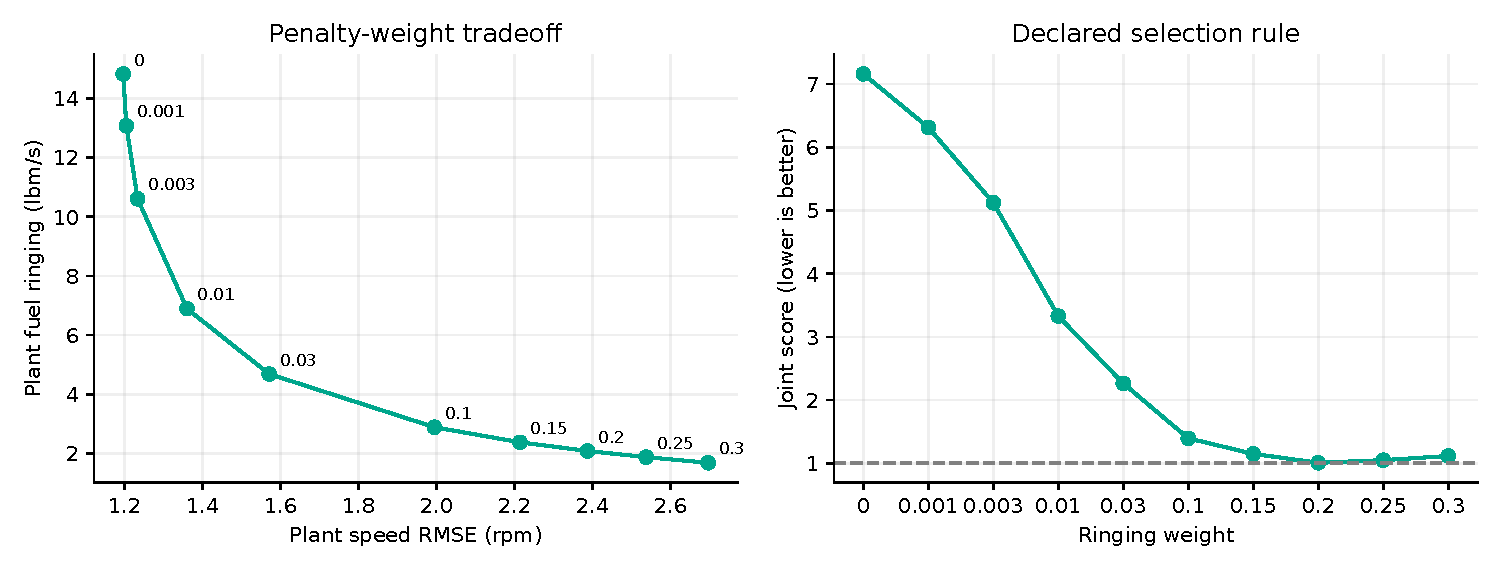
\includegraphics[width=\linewidth,height=.68\textheight,keepaspectratio]{late1_tradeoff.pdf}\caption{Measured 10\% plant tradeoff and the declared selection score. These are candidate evaluations, not independent validation.}\end{figure}

\subsection{Step 7: nonlinear results and interpretation}
The deployed gains are frozen at $K_p=0.02479762$, $K_i=0.05385920$ and $K_d=0$.
\begin{table}[H]\centering\small\begin{tabular}{lrrrr}\toprule
Controller & RMSE (rpm) & Peak (rpm) & Ringing & Settling (s)\\\midrule
Base PI & 2.4209 & 21.406 & 2.0702 & 2.475\\
Original Poly2 & 1.6658 & 14.113 & 1.6968 & 1.365\\
Retuned Poly2 & 1.5461 & 15.825 & 1.2990 & 0.930\\
Previous PILCO & 1.1973 & 14.389 & 14.8252 & 1.920\\
Smooth PILCO & 2.3877 & 21.593 & 2.0838 & 2.220\\\bottomrule\end{tabular}\caption{10\% load test. Ringing units are lbm/s; settling uses the persistent 0.1 rpm band.}\end{table}
\begin{table}[H]\centering\small\begin{tabular}{lrrrr}\toprule
Controller & RMSE (rpm) & Peak (rpm) & Ringing & Settling (s)\\\midrule
Base PI & 1.1692 & 10.392 & 1.0583 & 2.115\\
Original Poly2 & 0.8018 & 6.969 & 0.9005 & 1.260\\
Retuned Poly2 & 0.7439 & 7.806 & 0.6544 & 0.870\\
Previous PILCO & 0.5930 & 7.008 & 7.9471 & 1.695\\
Smooth PILCO & 1.1533 & 10.486 & 1.0615 & 1.905\\\bottomrule\end{tabular}\caption{5\% load test. Ringing units are lbm/s; settling uses the persistent 0.1 rpm band.}\end{table}
Relative to Base PI, smooth PILCO changes RMSE by -1.4\%, ringing by +0.7\%, and fine settling from 2.475 to 2.220 s.

Relative to Retuned Poly2, smooth PILCO changes RMSE by +54.4\%, ringing by +60.4\%, and fine settling from 0.930 to 2.220 s.

Relative to Previous PILCO, smooth PILCO changes RMSE by +99.4\%, ringing by -85.9\%, and fine settling from 1.920 to 2.220 s.

Its sampled peak fuel slew is 4.763 lbm/s$^2$, versus 10.514 for previous PILCO. Minimum surge margin changes from 14.800\% to 18.201\%; the selected 10\% run has 0.000\% fuel saturation. These diagnostics complement the objective rather than entering its selection score.

With the gains frozen, the 5\% test gives RMSE 1.1533 rpm and ringing 1.0615 lbm/s, a 86.6\% ringing reduction from previous PILCO. This supports amplitude transfer of the smoothing effect at this operating point.

\paragraph{What the video compares.} Four synchronized windows show base PI, retuned Poly2 + PID, previous PILCO, and smooth PILCO. Original Poly2 remains in the report tables but is omitted from the four-window video to make room for the new method. Each window has its own speed-error and fuel plots, matching axes, current speed, current fuel, a shaft-load indicator and full-test metrics. Orange shading marks load-on intervals. The video includes the full 10\% test, slowed load application/removal, frozen-gain 5\% validation and a final scorecard. All plotted values are recorded plant signals without visual smoothing.

\begin{figure}[H]\centering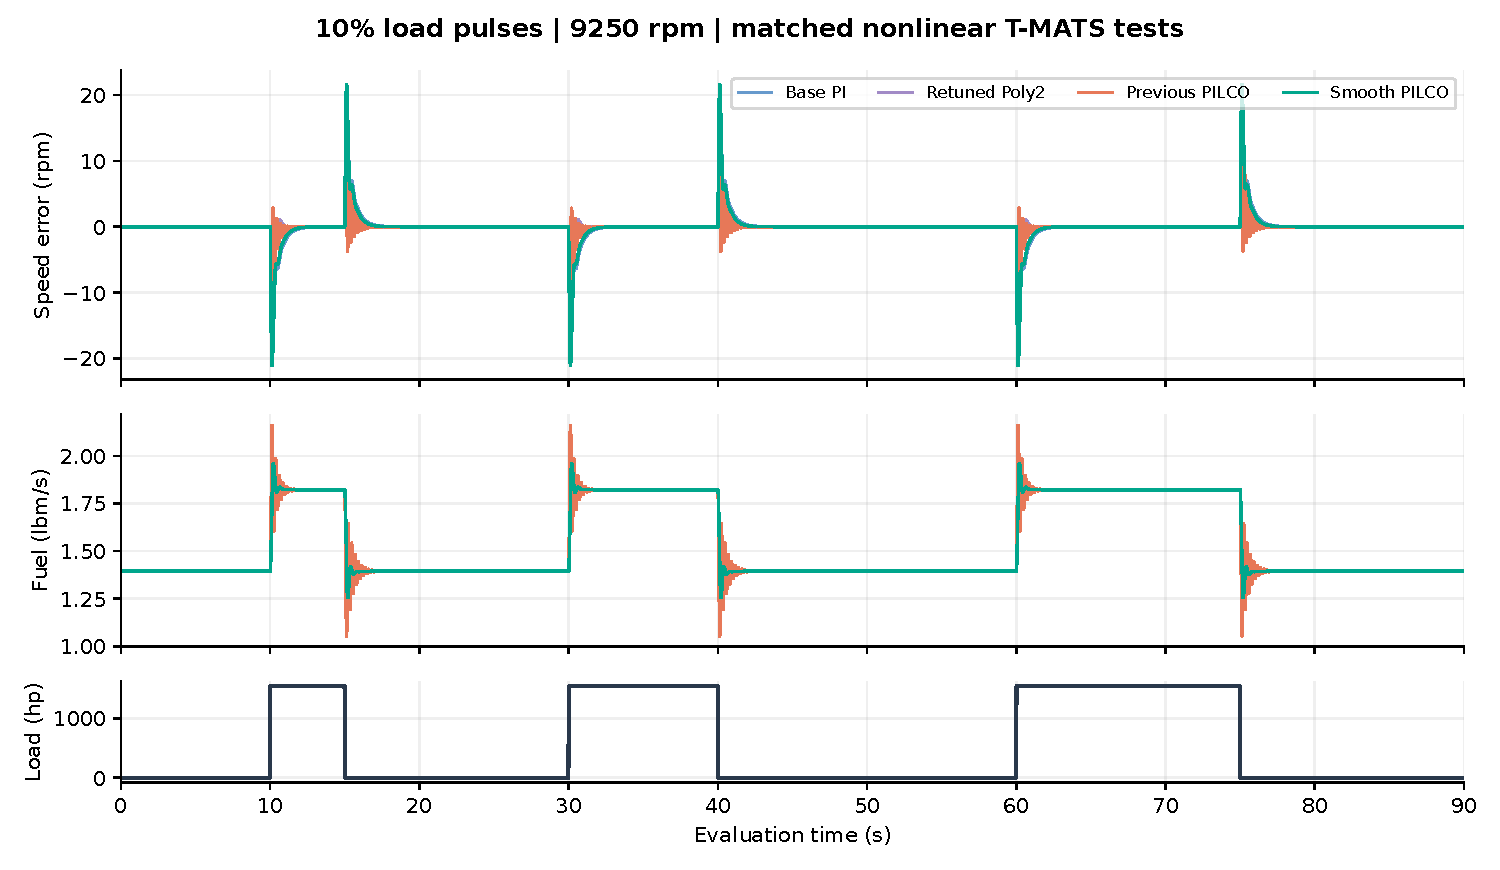
\includegraphics[width=\linewidth,height=.68\textheight,keepaspectratio]{late1_full_comparison.pdf}\caption{10\% full test; only the controller gains differ between the two PILCO policies.}\end{figure}
\begin{figure}[H]\centering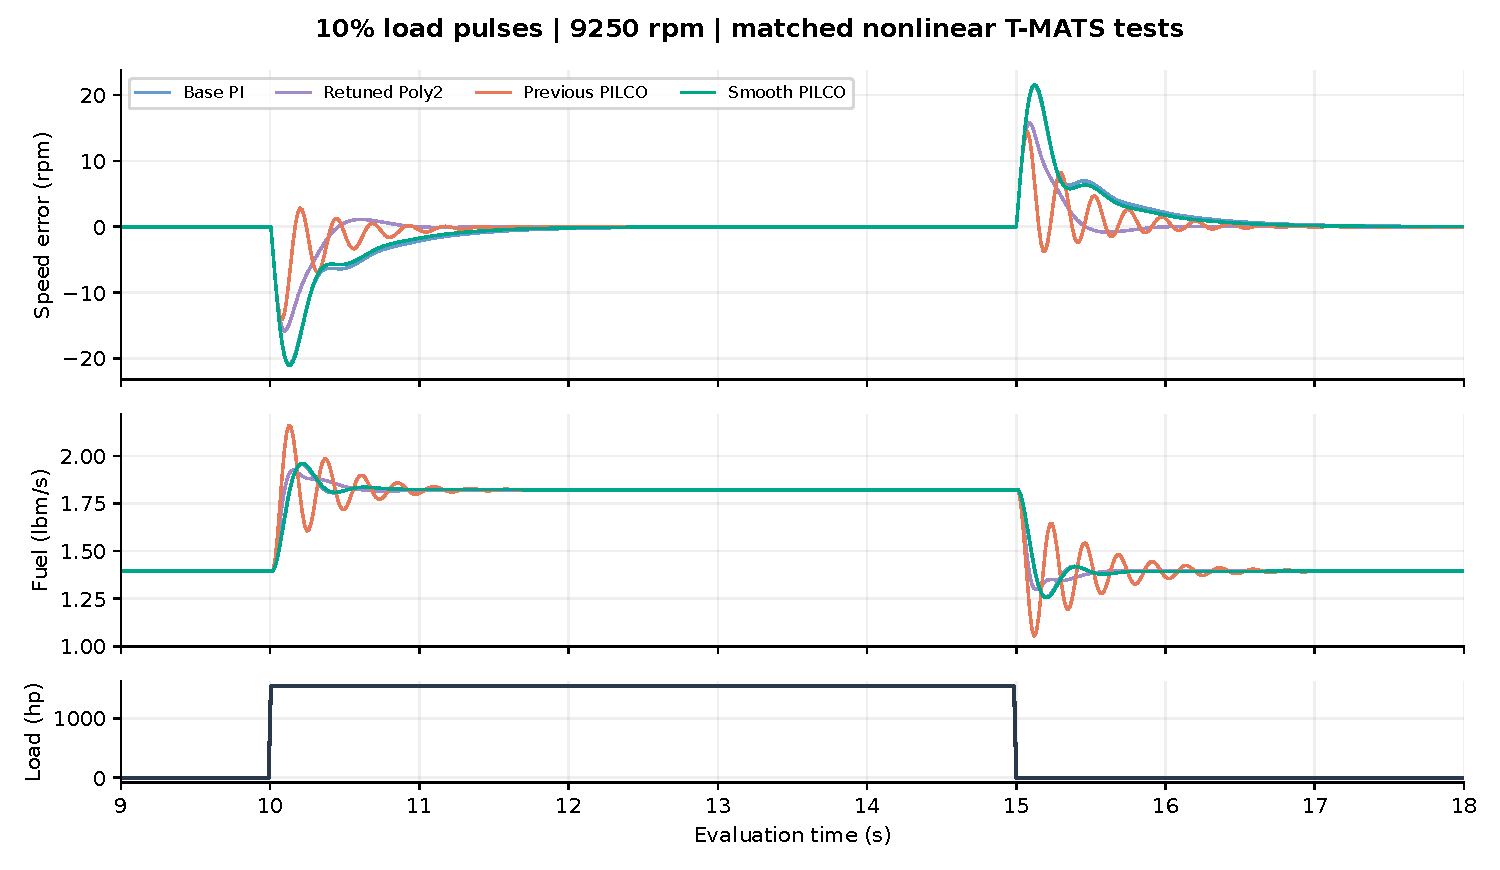
\includegraphics[width=\linewidth,height=.68\textheight,keepaspectratio]{late1_zoom_comparison.pdf}\caption{First load pulse, showing the effect of the ringing penalty on physical speed and fuel command.}\end{figure}
\begin{figure}[H]\centering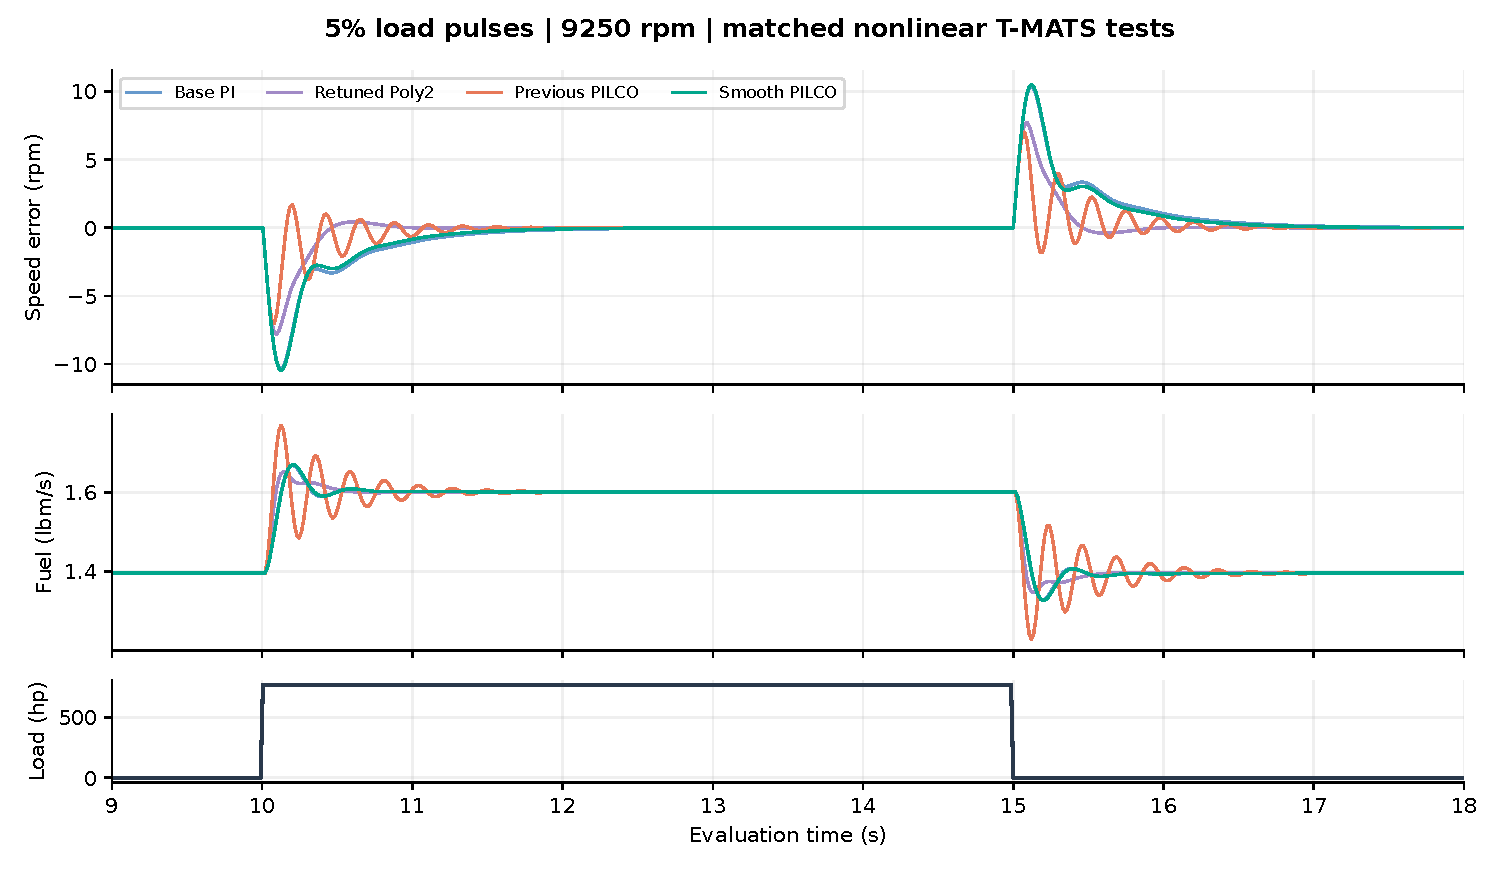
\includegraphics[width=\linewidth,height=.68\textheight,keepaspectratio]{late1_validation_comparison.pdf}\caption{Frozen-policy 5\% amplitude validation with the same timing and plant.}\end{figure}
\begin{figure}[H]\centering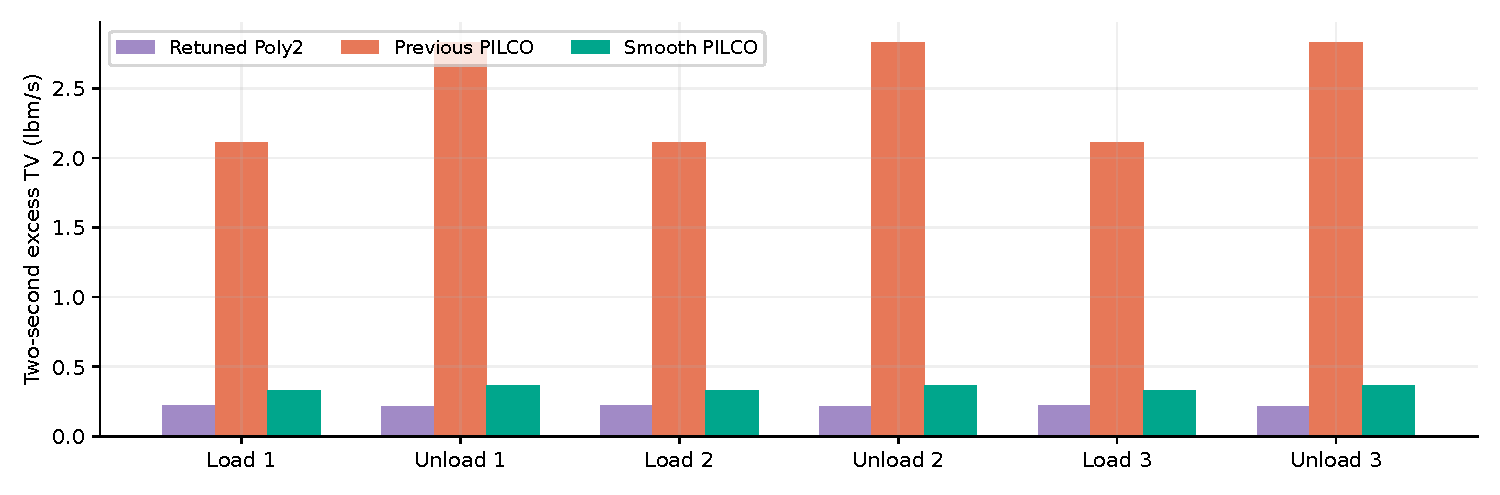
\includegraphics[width=\linewidth,height=.68\textheight,keepaspectratio]{late1_event_ringing.pdf}\caption{Ringing decomposed into six individual 10\% load edges. Each bar is total fuel movement minus net movement in the same two-second window.}\end{figure}

\subsection{Step 8: numerical checks and metric definitions}
All selected traces pass the shared plant acceptance checks. Maximum independent command replay discrepancy is 1.46e-13 lbm/s; maximum integral update discrepancy is 5.38e-15 lbm/s. The folded-normal formula passes 250,000-sample scalar Monte Carlo checks, including zero-variance and nonzero-variance cases. For the selected policy, a 5000-particle GP rollout predicts normalized excess TV 2.317963, compared with 2.317930 from Gaussian moment closure; their relative difference is 0.0014\%. The particle standard error is 0.000037. This checks prediction consistency on the same surrogate; it does not independently validate the physical GP uncertainty.

The plant acceptance test requires finite signals, positive fuel, positive surge margin, flow residual at most $10^{-9}$, fewer than 200 solver iterations, full 150 s duration and preparation speed within 0.1 rpm. Speed RMSE and peak error use all evaluation samples. IAE uses the previous study's rectangular sum. Ringing sums TV minus endpoint motion in six two-second load-edge windows. Fine settling requires staying inside $\pm0.1$ rpm until the next event; it is not a broad percentage-of-speed settling criterion. Reported peak slew is the maximum sampled fuel change divided by 0.015 s in those windows.

Independent replay reconstructs $u^*=u_{\rm ff}+K_p(r-N_s)+I$ and every eligible integral update, then checks the saved command. Metrics are recomputed from CSV and compared against MATLAB's shared implementation. Identical time, reference and load vectors are checked across compared runs. The extra previous-command and anchor states exist only in offline prediction: the runtime controller still requires just its integral state.

\subsection{Limits and how to use the result}
The result is smoother than the earlier tracking-only PILCO, but the complete comparison must also account for tracking, settling and surge margin. It does not dominate the retuned Poly2 controller on both speed RMSE and ringing. That comparator has derivative/acceleration feedback, whereas the new policy is restricted to PI. The chosen weight is the best under the declared score among the tested candidates, not a universal tuning value.

This is an offline PILCO-style method, not a reproduction of the original full collect--refit--improve loop. The original PILCO work motivates GP dynamics and uncertainty-aware policy evaluation~\cite{pilco}. This implementation uses a fitted linear mean, a subset GP with shared covariance hyperparameters, a restricted PI policy, numerical gradients, and a custom expected excess-TV cost. It assumes an unsaturated affine policy during planning; plant runs apply the actual saturation and anti-windup. Five-percent testing checks amplitude transfer at one operating point and is not proof of robustness to noise, speed changes, ambient changes or hardware dynamics.

To prioritize still less actuator activity, select a larger penalty only after examining its tracking cost. To require a hard slew bound, add and validate an explicit actuator-rate constraint or a different policy architecture; an excess-TV penalty alone does not provide such a bound. To claim advantages for the quadratic feedforward map itself, perform separate multi-speed and ambient validation.

\subsection{Reproduction}
Run \path{pilco_smooth.py} to load the frozen GP and optimize the coarse weights. Run \path{run_tmats_pilco_smooth('tune')} in MATLAB. Run \path{refine_pilco_smooth.py}, then repeat the MATLAB tuning call, which resumes saved candidates and evaluates the additions. Run \path{select_pilco_smooth.py} to write \path{selected_policy.json}, then \path{run_tmats_pilco_smooth('validate')} only after selection. The ready-to-open model is \path{GasTurbine_PILCO_Smooth_PI.mdl}; its preload callback loads the frozen selected policy. Run \path{check_pilco_smooth_mc.py} for the particle cross-check and the report/video builders for final artifacts. Outputs are in \path{results/pilco_smooth_20261010}. This is an overlay for the existing T-MATS workspace and adjacent library; earlier studies remain unchanged.



